\chapter{Other supporting analysis and graphs}

\section{Breakdown of tweets in full dataset}
\label{sec: apdxa_fulldataset}
\begin{table}[ht]
    \captionsetup{font=small}
    \small
    \centering
    \begin{tabularx}{\textwidth}{|X|c|c|c|}
        \hline
        \rowcolor[gray]{0.7}
        \textbf{Domains}            & \textbf{Complaints}            & \textbf{Non-Complaints}        & \textbf{Total Tweets} \\
        \hline
        Apparel                     & 145 \small{(55.3\%)}           & 117 \small{(44.7\%)}           & 262 \small{(7.6\%)}   \\
        \hline
        Cars                        & 68 \small{(73.1\%)}            & 25 \small{(26.9\%)}            & 93 \small{(2.7\%)}    \\
        \hline
        Electronics                 & 176 \small{(60.7\%)}           & 114 \small{(39.3\%)}           & 290 \small{(8.4\%)}   \\
        \hline
        Food \& Beverage            & 92 \small{(72.4\%)}            & 35 \small{(27.6\%)}            & 127 \small{(3.7\%)}   \\
        \hline
        Other                       & 95 \small{(74.2\%)}            & 33 \small{(25.8\%)}            & 128 \small{(3.7\%)}   \\
        \hline
        Retail                      & 122 \small{(61.9\%)}           & 75 \small{(38.1\%)}            & 197 \small{(5.7\%)}   \\
        \hline
        Services                    & 204 \small{(60.9\%)}           & 131 \small{(39.1\%)}           & 335 \small{(9.7\%)}   \\
        \hline
        Software \& Online Services & 192 \small{(65.1\%)}           & 103 \small{(34.9\%)}           & 295 \small{(8.6\%)}   \\
        \hline
        Transport                   & 138 \small{(55.9\%)}           & 109 \small{(44.1\%)}           & 247 \small{(7.2\%)}   \\
        \hline
        \rowcolor[gray]{0.9}
        \textbf{Sub-total}          & \textbf{1232 \small{(62.4\%)}} & \textbf{742 \small{(37.6\%)}}  & \textbf{1974}         \\
        \hline
        \hline
        Random Reply                & 0 \small{(0\%)}                & 739 \small{(100\%)}            & 739 \small{(21.4\%)}  \\
        \hline
        Random Tweet                & 0 \small{(0\%)}                & 736 \small{(100\%)}            & 736 \small{(21.3\%)}  \\
        \hline
        \hline
        \rowcolor[gray]{0.9}
        \textbf{Total}              & \textbf{1232 \small{(35.7\%)}} & \textbf{2217 \small{(64.3\%)}} & \textbf{3449}         \\
        \hline
    \end{tabularx}
    \caption{The nine domains and the distribution of tweets that are complaints and those that are not from the latest version of the dataset available in the public domain and for the experiments. Additionally, the table includes the number of random tweets and replies introduced into the dataset by the authors for a more proportionate representation of the classes.}
    \label{tab: fulldataset_breakdown}
\end{table}

\section{Sample data from dataset}
\begin{table}[ht]
    \captionsetup{font=small}
    \small
    \centering
    \begin{tabularx}{\textwidth}{|l|X|c|c|l|}
        \hline
        \rowcolor[gray]{0.7}
        \textbf{id} & \textbf{text}                                               & \textbf{binarylabel} & \textbf{multilabel} & \textbf{domain} \\
        \hline
        1.20E+17    & asus g60 series . bought it to play games but guess not bf3 & 1                    & 1                   & electronics     \\
        \hline
        4.88E+17    & love this trimmer ! making the sidewalk look sharp <url>    & 0                    & 0                   & other           \\
        \hline
    \end{tabularx}
    \caption{Sample data from \cite{jinModelingSeverityComplaints2021}.}
    \label{tab: apdx_sample_data}
\end{table}

The \texttt{binarylabel} represents the label for complaints with 1 indicating the tweet is a complaint. Columns \texttt{id} and \texttt{multilabel} are not used for the experiments.



\section{Token distribution after tokenization}
\label{sec: apdxa_token_dist}
The graphs in Figure \ref{fig: apdxa_tokens} show the distribution of token size for tweets from the full dataset for each of the models based on the tokenizer they use. The graph for BERT base uncased is in Chapter 3, Figure \ref{fig: bef_aft_token}.
\begin{figure}[htbp]
    \centering
    \captionsetup{font=small}
    \begin{subfigure}[b]{0.48\textwidth}
        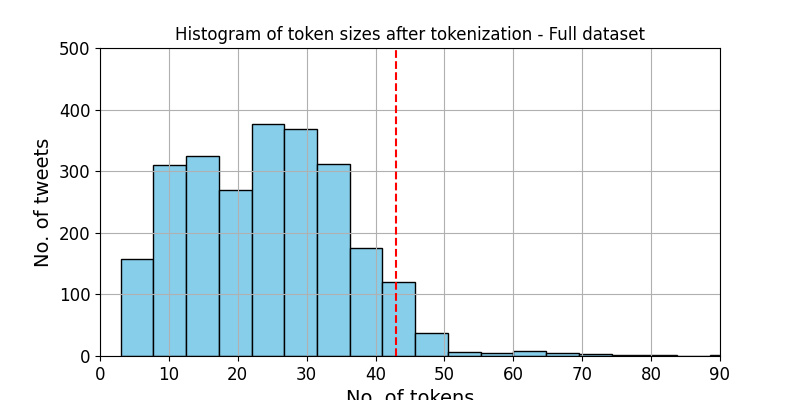
\includegraphics[width=\textwidth]{figures/token_pp_hist_albert-base-v2.png}
        \caption{AlBERT base}
        \label{fig: token_pp_hist_albert}
    \end{subfigure}
    \hfill
    \begin{subfigure}[b]{0.48\textwidth}
        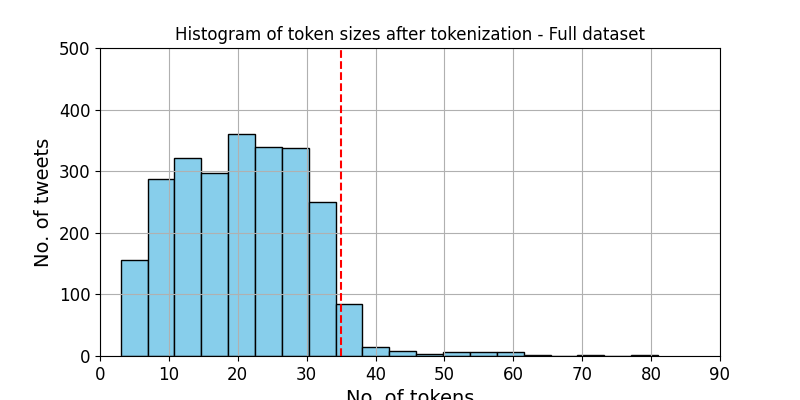
\includegraphics[width=\textwidth]{figures/token_pp_hist_vinai-bertweet-base.png}
        \caption{BERTweet}
        \label{fig: token_pp_hist_bertwteet}
    \end{subfigure}
    \begin{subfigure}[b]{0.48\textwidth}
        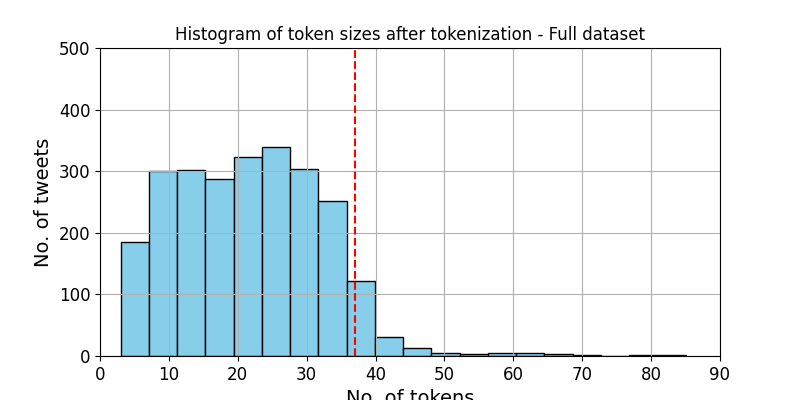
\includegraphics[width=\textwidth]{figures/token_pp_hist_prajjwal1-bert-tiny.png}
        \caption{BERT tiny}
        \label{fig: token_pp_hist_tiny}
    \end{subfigure}
    \hfill
    \begin{subfigure}[b]{0.48\textwidth}
        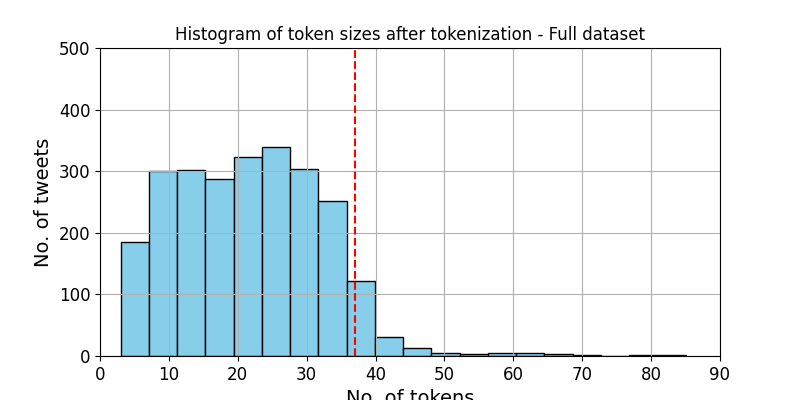
\includegraphics[width=\textwidth]{figures/token_pp_hist_distilbert-base-uncased.png}
        \caption{DistilBERT base uncased}
        \label{fig: token_pp_hist_distilbert}
    \end{subfigure}
    \begin{subfigure}[b]{0.48\textwidth}
        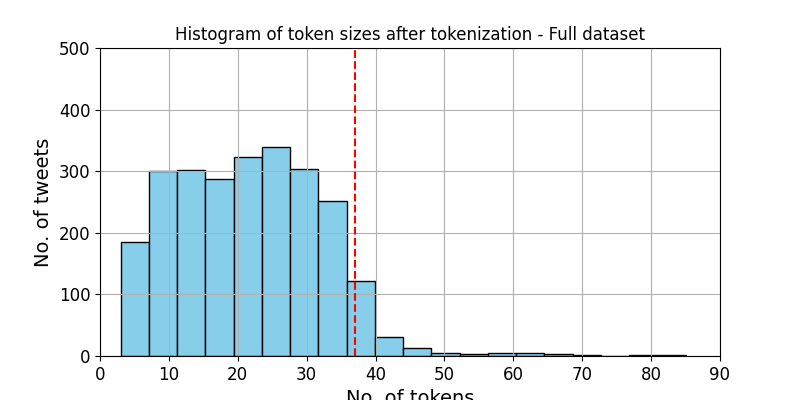
\includegraphics[width=\textwidth]{figures/token_pp_hist_google-mobilebert-uncased.png}
        \caption{MobileBERT uncased}
        \label{fig: token_pp_hist_mobile}
    \end{subfigure}
    \hfill
    \begin{subfigure}[b]{0.48\textwidth}
        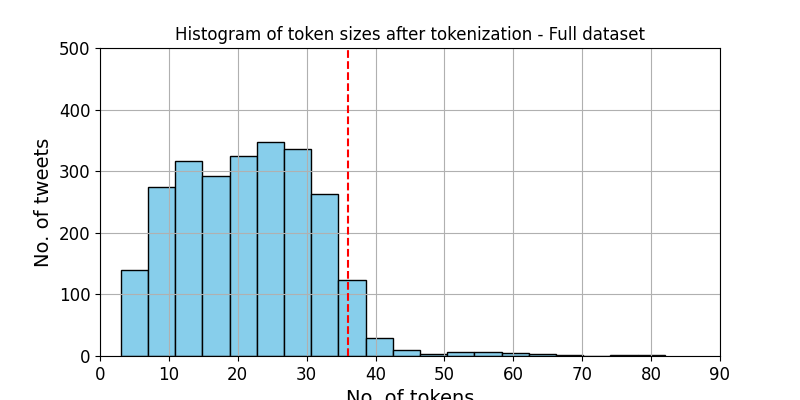
\includegraphics[width=\textwidth]{figures/token_pp_hist_roberta-base.png}
        \caption{RoBERTa base}
        \label{fig: token_pp_hist_roberta}
    \end{subfigure}
    \caption{The token count distribution for the full dataset of 3,449 tweets for all models.}
    \label{fig: apdxa_tokens}
\end{figure}

\subsection{Confusion matrix from every test run}
The elements of the matrix in left-to-right order are true negative, false positive, false negative and true positive.
\label{sec: conf_matrix_test_runs}
\begin{table}
    \centering
    \begin{tblr}{
      width = \linewidth,
      colspec = {Q[152]Q[283]Q[292]Q[194]},
      row{odd} = {Mercury},
      row{1} = {Nobel,c},
      column{1} = {c},
      cell{2}{2} = {c},
      cell{2}{3} = {c},
      cell{2}{4} = {c},
      cell{3}{2} = {c},
      cell{3}{3} = {c},
      cell{3}{4} = {c},
      cell{4}{2} = {c},
      cell{4}{3} = {c},
      cell{4}{4} = {c},
      cell{5}{2} = {c},
      cell{5}{3} = {c},
      cell{5}{4} = {c},
      cell{6}{2} = {c},
      cell{6}{3} = {c},
      cell{6}{4} = {c},
      cell{7}{2} = {c},
      cell{7}{3} = {c},
      cell{7}{4} = {c},
      hline{1-2,8} = {-}{},
      vlines,
    }
    \textbf{Test run} & \textbf{BERTweet Base}       & \textbf{DistilBERT Base}     & \textbf{BERT Tiny}           \\
    1                 & {{[}353~ ~17]\\{[} 22~ 183]} & {{[}350~ ~20]\\{[} 22~ 183]} & {{[}323~ ~47]\\{[} 74~ 131]} \\
    2                 & {{[}342~ ~28]\\{[} 12~ 193]} & {{[}330~ ~40]\\{[} 16~ 189]} & {{[}314~ ~56]\\{[} 84~ 121]} \\
    3                 & {{[}347~ ~23]\\{[} 18~ 187]} & {{[}356~ ~14]\\{[} 53~ 152]} & {{[}312~ ~58]\\{[} 83~ 122]} \\
    4                 & {{[}343~ ~26]\\{[} 12~ 194]} & {{[}335~ ~34]\\{[} 17~ 189]} & {{[}315~ ~54]\\{[} 67~ 139]} \\
    5                 & {{[}348~ ~21]\\{[} 24~ 182]} & {{[}330~ ~39]\\{[} 24~ 182]} & {{[}309~ ~60]\\{[} 88~ 118]} \\
    6                 & {{[}353~ ~16]\\{[} 10~ 195]} & {{[}354~ ~15]\\{[} 40~ 165]} & {{[}316~ ~53]\\{[} 64~ 141]} 
    \end{tblr}
    \caption{Confusion matrix from every test run for the experiments set 1.}
    \label{tab: conf_matrix_test_runs}    
\end{table}


